\documentclass[11pt,a4paper]{article}
\usepackage[utf8]{inputenc}
\usepackage[T1]{fontenc}
\usepackage[spanish,es-tabla]{babel}
\usepackage{amsmath,amssymb}
\usepackage{graphicx}
\usepackage{booktabs}
\usepackage{geometry}
\usepackage{hyperref}
\usepackage{float}
\usepackage[section]{placeins}

\geometry{margin=2.2cm}
\graphicspath{{../figuras/}{figuras/}}

\title{\textbf{Análisis modal y observabilidad en una cuerda 1D mediante esquema implícito y FFT}}
\author{Claudio Luis Campero \\ \small Laboratorio II -- Facultad de Ciencias Exactas, Universidad Nacional de Salta (UNSa)}
\date{Noviembre de 2026 \\ \small Repositorio: \href{https://github.com/claudioluis2002-droid/labo2-cuerda-fft}{\texttt{https://github.com/claudioluis2002-droid/labo2-cuerda-fft}}}

\begin{document}
\sloppy

\maketitle

\begin{abstract}
En este trabajo se estudia la vibración libre de una cuerda tensa homogénea de longitud $L = 1{,}00\text{ m}$ con extremos fijos, pulsada desde el reposo con un perfil triangular de altura $A = 5{,}0\text{ mm} \ll L$ en tres posiciones distintas ($a/L \in \{1/2, 1/3, 2/5\}$). Para resolver la ecuación de ondas unidimensional se dedujo e implementó un esquema implícito centrado de tres niveles temporales con matriz tridiagonal y arranque simétrico de segundo orden. Al verificar el código con un modo sinusoidal puro ($n=1$, $f_1 = 50\text{ Hz}$) y número de Courant $\sigma = 2{,}0$, el método se mantuvo estable, conservó la energía discreta con una variación relativa máxima de $2{,}47 \times 10^{-4}$ y presentó un error relativo de amplitud de $4{,}61 \times 10^{-5}$ y un error de fase de $5{,}23 \times 10^{-3}\text{ rad}$ al cabo de diez ciclos. Luego, combinando la serie de Fourier analítica con espectros FFT tomados en tres sensores virtuales ($x/L \in \{1/2, 1/3, 3/11\}$), se analizó cómo cambia la energía inicial al mover el punto de pulsación ($5{,}00\text{ mJ}$, $5{,}63\text{ mJ}$ y $5{,}21\text{ mJ}$) y cómo diferenciar un modo no excitado ($B_n = 0$) de un modo activo que no se detecta porque el sensor coincide con un nodo ($\sin(n\pi x_s/L) = 0$).
\end{abstract}

\section{Introducción}

El análisis espectral mediante transformada de Fourier permite estudiar los modos normales de vibración de una cuerda tensa a partir de mediciones temporales en uno o más puntos. En una cuerda ideal con extremos fijos, cualquier desplazamiento inicial libre puede escribirse como una suma de modos estacionarios con frecuencias propias $f_n = n c / (2L)$. Sin embargo, al observar el espectro obtenido en un punto de la cuerda, la ausencia de un pico puede deberse a dos causas diferentes: que ese modo no haya sido excitado por la forma inicial de la cuerda, o que el sensor esté ubicado justo sobre un nodo de ese modo.

El objetivo de este trabajo es estudiar cómo cambia la distribución de amplitud y energía entre los modos normales al desplazar el vértice de una pulsación triangular ($a/L = 1/2, 1/3, 2/5$) manteniendo fija la altura inicial, y distinguir mediante análisis FFT qué armónicos faltan por falta de excitación y cuáles no se ven por la posición del sensor ($x/L = 1/2, 1/3, 3/11$).

\section{Metodología}

\subsection{Modelo físico y referencia analítica}

Se modela una cuerda homogénea de longitud $L = 1{,}00\text{ m}$, tensión $\mathcal{T} = 100{,}0\text{ N}$ y densidad lineal $\mu = 0{,}010\text{ kg/m}$. Con estos valores, la velocidad de propagación transversal es $c = \sqrt{\mathcal{T}/\mu} = 100{,}0\text{ m/s}$ y la frecuencia fundamental es $f_1 = c/(2L) = 50{,}0\text{ Hz}$. Bajo la hipótesis de pequeñas deformaciones ($A/L = 5 \times 10^{-3} \ll 1$), el desplazamiento $y(x,t)$ cumple la ecuación de ondas 1D:
\begin{equation}
\frac{\partial^2 y}{\partial t^2} = c^2 \frac{\partial^2 y}{\partial x^2}, \qquad x \in (0,L),\; t > 0,
\label{eq:onda_1d}
\end{equation}
con extremos fijos $y(0,t) = y(L,t) = 0$, velocidad inicial nula $\partial_t y(x,0) = 0$ y deformación inicial triangular de amplitud $A = 5{,}0\text{ mm}$ con vértice en $x = a$:
\begin{equation}
y(x,0) = f(x) = \begin{cases}
\dfrac{A}{a}\,x, & 0 \le x \le a, \\[6pt]
\dfrac{A}{L - a}\,(L - x), & a < x \le L.
\end{cases}
\label{eq:triangular}
\end{equation}

Para contrastar los resultados numéricos se usa la solución analítica en serie de Fourier truncada a $N_{\text{modos}} = 200$ términos (deducida en el Apéndice~\ref{ap:coeficientes_bn}):
\begin{equation}
y_{\text{ref}}(x,t) = \sum_{n=1}^{N_{\text{modos}}} B_n \sin\left(\frac{n\pi x}{L}\right) \cos\left(\frac{n\pi c}{L}t\right), \qquad B_n = \frac{2 A L^2}{n^2 \pi^2 a (L - a)} \sin\left(\frac{n\pi a}{L}\right).
\label{eq:sol_referencia}
\end{equation}
Aunque la altura máxima $A$ sea la misma en todos los casos y se mantenga fija la tensión $\mathcal{T}$, la energía mecánica inicial $E_0(a) = \mathcal{T}A^2 L / [2a(L-a)]$ cambia con la posición del vértice $a$ y toma su valor mínimo cuando se pulsa en el centro ($a/L = 1/2$).

\subsection{Método numérico y análisis espectral}

El espacio se divide en $N_x = 660$ intervalos iguales ($\Delta x = L/660 \approx 1{,}515\text{ mm}$). Se eligió $660$ por ser múltiplo de $2, 3, 5$ y $11$, de modo que tanto los puntos de pulsación como los sensores caen exactamente sobre nodos de la grilla sin necesidad de interpolar. Para avanzar en el tiempo se dedujo un esquema implícito centrado de tres niveles con pesos $(1/4, 1/2, 1/4)$ en espacio (Apéndice~\ref{ap:esquema_implicito}), que lleva en cada paso $n \to n+1$ al sistema tridiagonal:
\begin{equation}
-\frac{\sigma^2}{4} y_{i-1}^{n+1} + \left(1 + \frac{\sigma^2}{2}\right) y_i^{n+1} - \frac{\sigma^2}{4} y_{i+1}^{n+1} = 2y_i^n - y_i^{n-1} + \frac{\sigma^2}{4}\left(2\delta_x^2 y_i^n + \delta_x^2 y_i^{n-1}\right),
\label{eq:esquema_cuerpo}
\end{equation}
donde $\sigma = c\Delta t/\Delta x$ es el número de Courant. En las primeras pruebas se vio que arrancar desde el reposo ($y_i^{-1} = y_i^1$) con la fórmula explícita de Taylor ($y_i^1 = y_i^0 + \frac{\sigma^2}{2}\delta_x^2 y_i^0$) funciona bien para ondas suaves, pero falla en el perfil triangular cuando $\sigma = 6{,}6 > 1$ porque multiplica el cambio brusco de pendiente en el vértice $x = a$. Por eso, el primer paso $n = 1$ se resolvió también de forma implícita imponiendo simetría temporal~\cite{gutierrez} (Apéndice~\ref{ap:primer_paso}):
\begin{equation}
\left(I - \frac{\sigma^2}{4} D_2\right)\mathbf{y}^1 = \left(I + \frac{\sigma^2}{4} D_2\right)\mathbf{y}^0.
\label{eq:arranque_cuerpo}
\end{equation}

El programa está escrito en Python (\texttt{codigo/simulacion\_cuerda.py}) y resuelve el sistema tridiagonal en cada paso mediante \texttt{scipy.linalg.solve\_banded}, para lograr una mayor eficiencia que \texttt{np.linalg.solve}. Para las simulaciones principales se tomó $\Delta t = 1{,}0 \times 10^{-4}\text{ s}$ ($f_s = 10\text{ kHz}$, con frecuencia de Nyquist $f_{\text{Nyq}} = 5\text{ kHz} \gg f_{10} = 500\text{ Hz}$, evitando \textit{aliasing}) durante un tiempo total $T_{\text{tot}} = 1{,}00\text{ s}$ ($N = 10\,000$ muestras), lo que da una resolución en frecuencia $\Delta f = 1/T_{\text{tot}} = 1{,}0\text{ Hz}$. A cada señal centrada se le aplicó una ventana de Hann (\texttt{np.hanning(N)}) para reducir las fugas espectrales y se dividió por su factor de ganancia coherente ($\langle w \rangle = 0{,}5$) multiplicando por $2/N$ para obtener las amplitudes en milímetros.

\section{Resultados}

\subsection{Verificación del esquema numérico con modo sinusoidal único}

Antes de simular el perfil triangular, se probó el código con un único modo normal $y(x,0) = A\sin(\pi x/L)$ ($f_1 = 50\text{ Hz}$) durante $t = 0{,}20\text{ s}$ ($10$ períodos). Con $N_x = 200$ y $\Delta t = 1{,}0 \times 10^{-4}\text{ s}$, el número de Courant vale $\sigma = 2{,}0$, un régimen donde los métodos explícitos son inestables. Como se observa en la Figura~\ref{fig:verificacion} (izquierda), la solución implícita se mantiene estable y conserva la energía discreta con una variación relativa máxima de $2{,}47 \times 10^{-4}$ (Apéndice~\ref{ap:energia_discreta}). Ajustando una sinusoide en los últimos dos ciclos se separaron los errores de amplitud y fase: el error relativo de amplitud es $4{,}61 \times 10^{-5}$ (el esquema no disipa amplitud) y el error de fase acumulado es $5{,}23 \times 10^{-3}\text{ rad}$ ($0{,}30^\circ$), debido a la dispersión numérica de la malla espacial.

\begin{figure}[htbp]
\centering
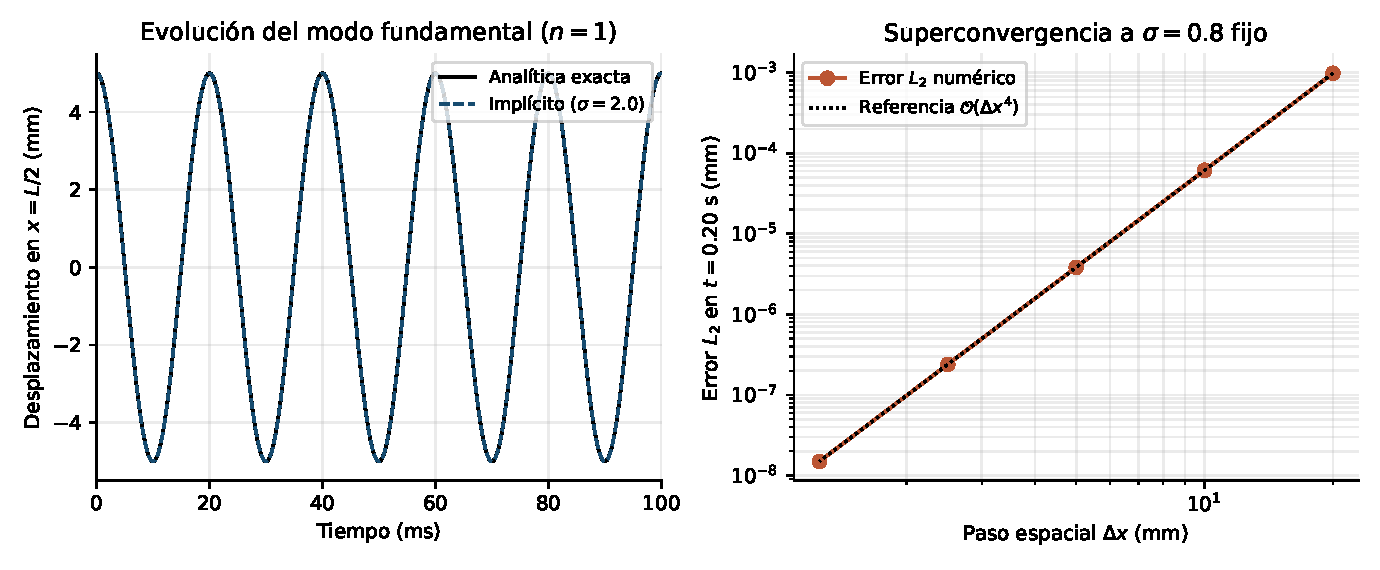
\includegraphics[width=0.86\textwidth]{fig1_verificacion_modo1.pdf}
\caption{Verificación del esquema implícito frente a la solución exacta del modo fundamental ($n=1$, $f_1=50\text{ Hz}$). Izquierda: desplazamiento en $x=L/2$ para $\sigma = 2{,}0$. Derecha: error $L_2$ en $t = 0{,}20\text{ s}$ al refinar la malla espacial $N_x \in \{50, 100, 200, 400, 800\}$.}
\label{fig:verificacion}
\end{figure}

El refinamiento de malla a número de Courant fijo ($\sigma = 0{,}8$, Figura~\ref{fig:verificacion} derecha) muestra que, aunque el esquema es formalmente de orden $\mathcal{O}(\Delta x^2 + \Delta t^2)$, en 1D los términos dominantes de dispersión espacial y temporal se compensan parcialmente y el error $L_2$ cae con superconvergencia de cuarto orden ($\mathcal{O}(\Delta x^4)$, datos en \texttt{resultados/verificacion\_refinamiento.csv}).

\subsection{Excitación modal y energía inicial según el punto de pulsación}

La Tabla~\ref{tab:coeficientes} y la Figura~\ref{fig:excitacion} (izquierda) muestran los coeficientes analíticos $B_n$ de los primeros diez modos según~\eqref{eq:sol_referencia}. Al mover el punto de pulsación $a/L$, cambian los modos que reciben energía:
\begin{itemize}
\item En $a/L = 1/2$, $\sin(n\pi/2) = 0$ para todo $n$ par, por lo que no se excita ningún modo par ($n = 2, 4, 6, 8, 10$).
\item En $a/L = 1/3$, $\sin(n\pi/3) = 0$ cuando $n$ es múltiplo de $3$, anulándose $n = 3, 6, 9$.
\item En $a/L = 2/5$, $\sin(2n\pi/5) = 0$ cuando $n$ es múltiplo de $5$, anulándose $n = 5, 10$.
\end{itemize}

\begin{table}[htbp]
\centering
\caption{Frecuencias propias $f_n$ y coeficientes modales analíticos $B_n$ (en mm) para los primeros diez modos según el punto de pulsación $a/L$ ($A = 5{,}0\text{ mm}$). Datos guardados en \texttt{resultados/coeficientes\_modales\_Bn.csv}.}
\label{tab:coeficientes}

\begin{tabular}{rrrrr}
\toprule
Modo $n$ & $f_n$ (Hz) & $B_n$ ($a/L=1/2$) [mm] & $B_n$ ($a/L=1/3$) [mm] & $B_n$ ($a/L=2/5$) [mm] \\
\midrule
1 & 50 & $+4{,}0528$ & $+3{,}9486$ & $+4{,}0151$ \ \\
2 & 100 & $0{,}0000$ & $+0{,}9872$ & $+0{,}6204$ \ \\
3 & 150 & $-0{,}4503$ & $0{,}0000$ & $-0{,}2757$ \ \\
4 & 200 & $0{,}0000$ & $-0{,}2468$ & $-0{,}2509$ \ \\
5 & 250 & $+0{,}1621$ & $-0{,}1579$ & $0{,}0000$ \ \\
6 & 300 & $0{,}0000$ & $0{,}0000$ & $+0{,}1115$ \ \\
7 & 350 & $-0{,}0827$ & $+0{,}0806$ & $+0{,}0506$ \ \\
8 & 400 & $0{,}0000$ & $+0{,}0617$ & $-0{,}0388$ \ \\
9 & 450 & $+0{,}0500$ & $0{,}0000$ & $-0{,}0496$ \ \\
10 & 500 & $0{,}0000$ & $-0{,}0395$ & $0{,}0000$ \ \\
\bottomrule
\end{tabular}
\end{table}
La Figura~\ref{fig:excitacion} (derecha) muestra además que la energía mecánica inicial no es igual en los tres casos: vale $E_0(1/2) = 5{,}00\text{ mJ}$ (discreta: $4{,}93\text{ mJ}$), sube a $E_0(2/5) = 5{,}21\text{ mJ}$ (discreta: $5{,}13\text{ mJ}$) y alcanza $E_0(1/3) = 5{,}63\text{ mJ}$ (discreta: $5{,}53\text{ mJ}$), conservándose en toda la simulación con variación relativa menor a $1{,}5 \times 10^{-3}$.
\begin{figure}[htbp]
\centering
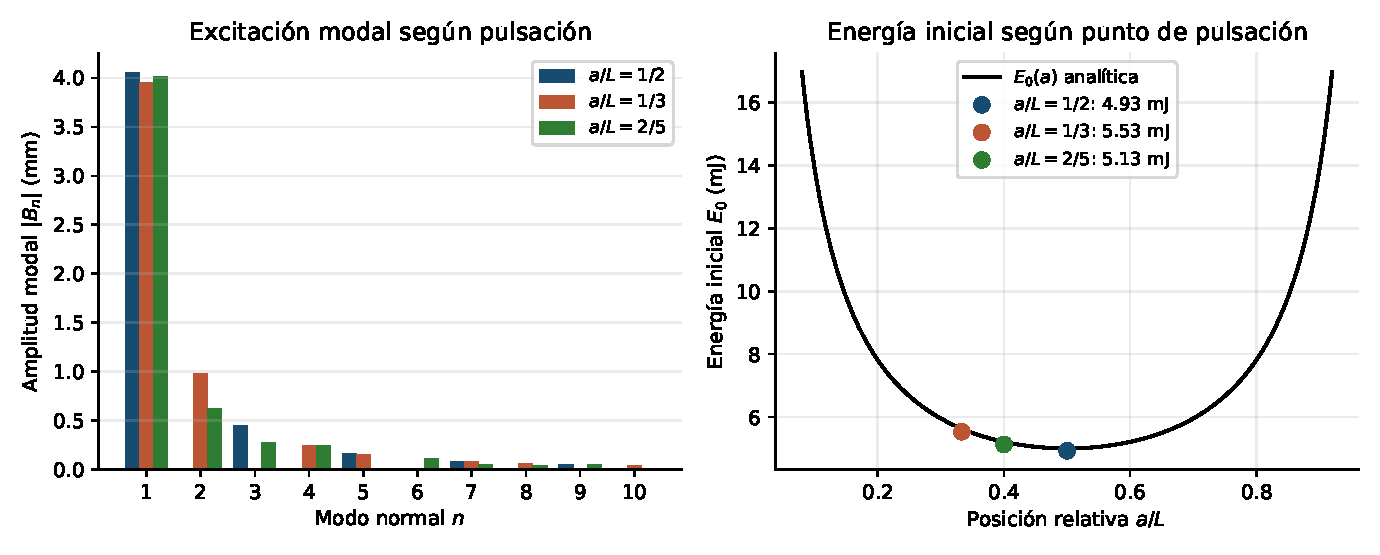
\includegraphics[width=0.86\textwidth]{fig2_excitacion_y_energia.pdf}
\caption{Izquierda: magnitud de los coeficientes modales $|B_n|$ para los tres puntos de pulsación. Derecha: energía potencial inicial analítica $E_0(a)$ comparada con la energía discreta inicial de cada simulación ($A = 5{,}0\text{ mm}$).}
\label{fig:excitacion}
\end{figure}
\subsection{Espectros FFT, observabilidad y comparación temporal}
La Figura~\ref{fig:espectros} muestra los espectros de amplitud obtenidos por FFT para las tres posiciones de pulsación (filas) y los tres sensores virtuales (columnas). Todos los picos aparecen en las frecuencias propias $f_n = 50n\text{ Hz}$, pero la presencia o ausencia de cada pico depende de dónde se mida:
\begin{enumerate}
\item En el sensor central $x/L = 1/2$ (primera columna), no aparece ningún modo par ($100, 200, 300, 400, 500\text{ Hz}$) en ninguno de los tres casos, porque $x/L = 1/2$ es un nodo de todos los modos pares. Sin embargo, al pulsar en $a/L = 1/3$ o $2/5$, los modos $n=2$ ($100\text{ Hz}$) y $n=4$ ($200\text{ Hz}$) sí están presentes y se ven claramente en los sensores $x/L = 1/3$ y $x/L = 3/11$.
\item En el sensor $x/L = 1/3$ (segunda columna), faltan siempre los múltiplos de $3$ ($150, 300, 450\text{ Hz}$). Por ejemplo, cuando se pulsa en el centro ($a/L = 1/2$, primera fila), el modo $n=3$ ($150\text{ Hz}$) sí tiene energía ($|B_3| = 0{,}45\text{ mm}$, visible en $x/L = 1/2$ y $3/11$), pero resulta invisible en $x/L = 1/3$ porque allí tiene un nodo.
\item El sensor $x/L = 3/11$ (tercera columna) no coincide con ningún nodo para $n < 11$, por lo que detecta todos los modos activos en cada caso.
\end{enumerate}
\begin{figure}[htbp]
\centering
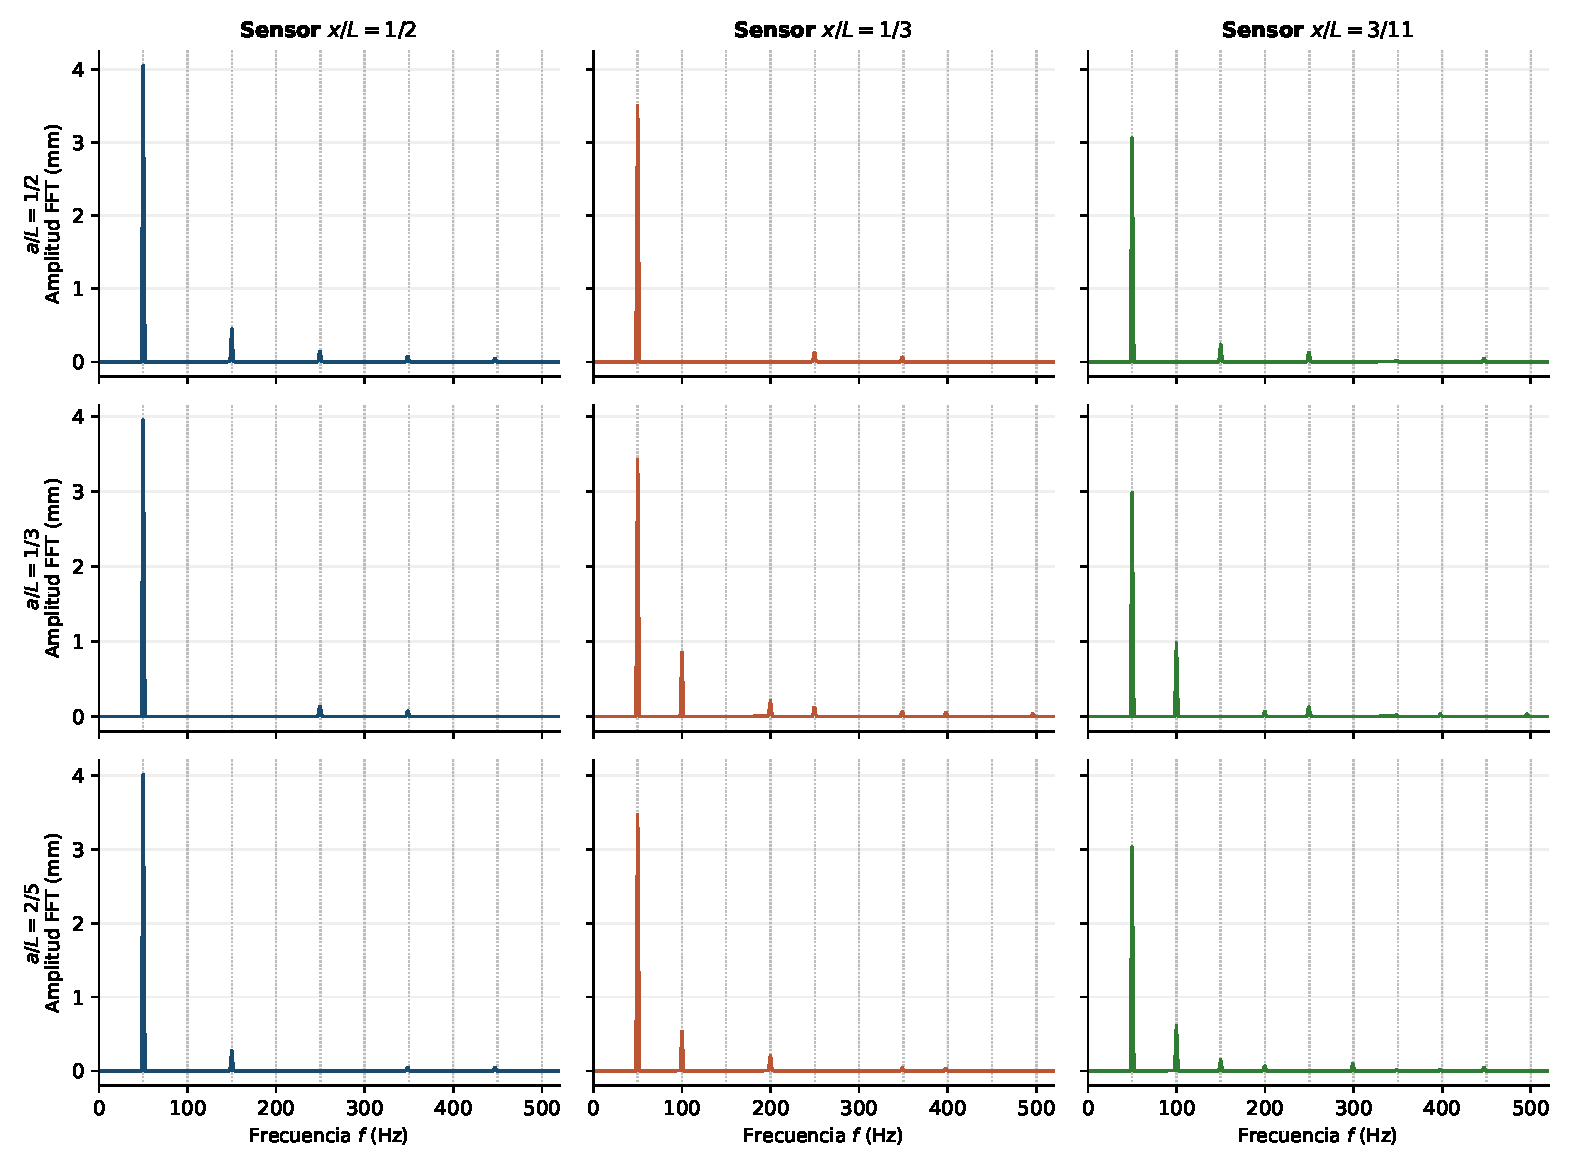
\includegraphics[width=0.88\textwidth]{fig3_espectros_observabilidad.pdf}
\caption{Espectros FFT hasta $520\text{ Hz}$ para las nueve combinaciones de punto de pulsación $a/L$ (filas) y posición de sensor $x/L$ (columnas). Las líneas verticales punteadas indican las frecuencias propias $f_n = 50n\text{ Hz}$.}
\label{fig:espectros}
\end{figure}

El error cuadrático medio (RMS) en $1{,}0\text{ s}$ se mantiene entre $0{,}12\text{ mm}$ y $0{,}25\text{ mm}$ en todos los sensores, concentrándose las diferencias en el paso del vértice agudo debido al retardo de fase por dispersión numérica de los armónicos más altos (mientras que en los espectros FFT el uso de ventana de Hann centrada en $T_{\text{tot}}/2$ introduce un salto de fase determinista de $\pi$ entre bines consecutivos que no altera las amplitudes modales).

\begin{figure}[htbp]
\centering
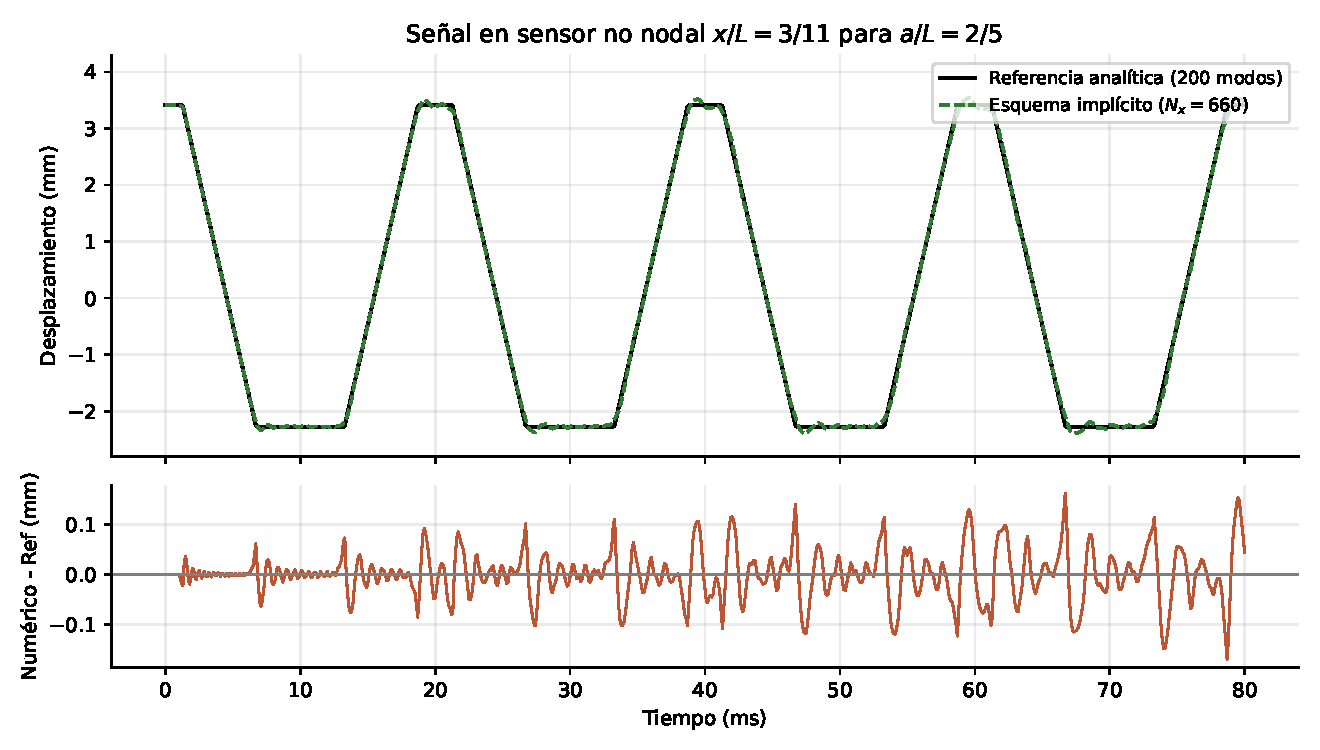
\includegraphics[width=0.86\textwidth]{fig4_comparacion_temporal.pdf}
\caption{Comparación temporal entre el esquema implícito ($N_x=660$, $\Delta t = 10^{-4}\text{ s}$) y la referencia analítica ($200$ modos) en $x/L = 3/11$ para $a/L = 2/5$ (arriba) y diferencia punto a punto (abajo).}
\label{fig:temporal}
\end{figure}
\section{Discusión}
Los espectros obtenidos muestran que la amplitud medida en un sensor ubicado en $x_s$ depende del producto $B_n \sin(n\pi x_s/L)$, lo que permite distinguir dos situaciones distintas cuando falta una frecuencia:
\begin{itemize}
\item \textbf{Modo no excitado ($B_n = 0$):} Ocurre cuando el punto de pulsación $a$ coincide con un nodo del modo $n$ ($\sin(n\pi a/L) = 0$). Ese modo no recibe energía y no aparecerá en ningún sensor.
\item \textbf{Modo no observado ($\sin(n\pi x_s/L) = 0$ con $B_n \neq 0$):} Ocurre cuando el modo sí está vibrando, pero el sensor se colocó en uno de sus nodos. Usando al menos dos sensores en posiciones no redundantes (como $x/L = 1/2$ y $x/L = 1/3$) o un sensor no nodal como $x/L = 3/11$, se pueden observar todos los modos excitados hasta $n = 10$.
\end{itemize}
Un aspecto importante observado durante el desarrollo del código fue el cálculo del primer paso temporal ($n = 1$). Aunque el arranque explícito de Taylor conserva la energía en el modo sinusoidal suave, al aplicarlo al perfil triangular con $\Delta x = L/660$ y $\Delta t = 10^{-4}\text{ s}$ ($\sigma = 6{,}6$), el salto de pendiente en el vértice $x = a$ queda multiplicado por $\sigma^2/2 = 21{,}78$. Esto hace que el vértice sobrepase su posición e inyecte energía cinética artificial ($E \approx 45\,E_0$, con deriva relativa de $44{,}7$), produciendo oscilaciones parásitas sobre las mesetas de la onda. Al reemplazar ese paso por el arranque implícito simétrico~\eqref{eq:arranque_cuerpo}, esta aproximación suaviza la esquina desde $t = 0$, la energía se conserva dentro del $0{,}15\%$ y desaparece el ruido numérico.
Finalmente, el esquema implícito centrado conserva la amplitud sin amortiguamiento artificial, aunque presenta dispersión numérica (retardo de fase) en las longitudes de onda más cortas, lo que explica el residuo localizado junto a las esquinas del triángulo en la Figura~\ref{fig:temporal}. Además, el modelo lineal~\eqref{eq:onda_1d} no incluye amortiguamiento viscoso con el aire, pérdidas en los soportes ni rigidez a la flexión, efectos que en una cuerda real atenuarían progresivamente los armónicos altos.
\section{Conclusiones}
Se implementó y verificó un esquema implícito conservativo de segundo orden para simular la vibración libre de una cuerda 1D pulsada triangularmente. Se comprobó que al desplazar el punto de pulsación $a/L$ de $1/2$ a $2/5$ y $1/3$, la energía inicial aumenta de $5{,}00\text{ mJ}$ a $5{,}21\text{ mJ}$ y $5{,}63\text{ mJ}$, y se suprimen distintas familias de armónicos según $\sin(n\pi a/L)$. El análisis FFT en múltiples sensores permitió diferenciar con claridad los modos no excitados de los modos ocultos por coincidencia nodal, verificando que la combinación de sensores coprimos recupera todo el espectro activo.
\begin{thebibliography}{9}
\bibitem{gutierrez} J. Gutierrez, \textit{Material de cátedra, guías y apuntes de Trabajo Final -- Laboratorio II}, Facultad de Ciencias Exactas, Universidad Nacional de Salta (UNSa), 2026.
\bibitem{repo} C. L. Campero, \textit{Repositorio reproducible del Trabajo Final -- Laboratorio II (UNSa)}, \href{https://github.com/claudioluis2002-droid/labo2-cuerda-fft}{\texttt{https://github.com/claudioluis2002-droid/labo2-cuerda-fft}}, carpeta \texttt{codigo/simulacion\_cuerda.py}, 2026.
\end{thebibliography}
\appendix
\section{Deducción del esquema implícito y sistema tridiagonal}
\label{ap:esquema_implicito}

Partiendo de la ecuación de ondas~\eqref{eq:onda_1d} y del esquema de diferencias finitas con matrices tridiagonales de la cátedra~\cite{gutierrez}, donde se discretiza $[0,L]$ con paso $\Delta x = L/N_x$ ($x_i = i\Delta x$) y el tiempo con paso $\Delta t$ ($t_n = n\Delta t$), aproximamos la ecuación~\eqref{eq:onda_1d} en $(x_i, t_n)$ mediante diferencias centradas en tiempo y un promedio ponderado $(1/4, 1/2, 1/4)$ de la segunda diferencia espacial $\delta_x^2 y_i^n = y_{i+1}^n - 2y_i^n + y_{i-1}^n$:

\begin{equation}
\frac{y_i^{n+1} - 2y_i^n + y_i^{n-1}}{\Delta t^2} = \frac{c^2}{4\Delta x^2}\left(\delta_x^2 y_i^{n+1} + 2\delta_x^2 y_i^n + \delta_x^2 y_i^{n-1}\right).
\end{equation}
Definiendo $\sigma = c\Delta t/\Delta x$ y agrupando las incógnitas del nivel $n+1$ a la izquierda, resulta para $i = 1, \dots, N_x - 1$:
\begin{equation}
-\frac{\sigma^2}{4} y_{i-1}^{n+1} + \left(1 + \frac{\sigma^2}{2}\right) y_i^{n+1} - \frac{\sigma^2}{4} y_{i+1}^{n+1} = 2y_i^n - y_i^{n-1} + \frac{\sigma^2}{4}\left(2\delta_x^2 y_i^n + \delta_x^2 y_i^{n-1}\right),
\end{equation}
con $y_0^{n+1} = y_{N_x}^{n+1} = 0$. La matriz resultante de dimensión $(N_x - 1) \times (N_x - 1)$ es tridiagonal, simétrica y estrictamente diagonal dominante ($1 + \sigma^2/2 > \sigma^2/2$), resolviéndose en $\mathcal{O}(N_x)$ operaciones.
\section{Deducción del primer paso temporal ($n = 1$)}
\label{ap:primer_paso}
Como el esquema general utiliza tres niveles temporales ($n+1$, $n$, $n-1$), para calcular el primer paso ($n=1$) se requiere conocer el estado ficticio $y_i^{-1}$ en $t = -\Delta t$. Siguiendo la metodología de la guía de cátedra~\cite{gutierrez} para condiciones iniciales en reposo, se aproxima la derivada temporal $\partial_t y(x_i, 0) = 0$ mediante una diferencia finita centrada en $t = 0$, lo que establece la simetría $y_i^{-1} = y_i^1$. A diferencia del desarrollo explícito de Taylor de la guía, aquí dicha simetría ($(y_i^1 - y_i^{-1})/(2\Delta t) = 0 \implies y_i^{-1} = y_i^1$) se sustituye directamente dentro de la ecuación implícita del Apéndice~\ref{ap:esquema_implicito} evaluada en $n=0$, manteniendo así la misma matriz tridiagonal y la estabilidad incondicional desde el instante inicial:

\begin{equation}
2(y_i^1 - y_i^0) = \frac{\sigma^2}{4}\left(2\delta_x^2 y_i^1 + 2\delta_x^2 y_i^0\right) \implies \left(1 - \frac{\sigma^2}{4}\delta_x^2\right)y_i^1 = \left(1 + \frac{\sigma^2}{4}\delta_x^2\right)y_i^0.
\end{equation}
Este arranque conserva la estructura tridiagonal del paso general, es de orden $\mathcal{O}(\Delta t^2, \Delta x^2)$ y evita amplificar la discontinuidad de pendiente del vértice triangular.
\section{Conservación de la energía mecánica discreta}
\label{ap:energia_discreta}
La expresión de la energía mecánica discreta proviene de discretizar directamente la integral de energía total de una cuerda tensa continua, $E(t) = \frac{1}{2}\int_0^L [\mu(\partial_t y)^2 + \mathcal{T}(\partial_x y)^2]\,dx$, evaluando la velocidad mediante diferencias hacia adelante entre $t_n$ y $t_{n+1}$ y la energía elástica mediante el producto cruzado de las pendientes discretas en ambos niveles temporales. Para demostrar su conservación exacta (analogía discreta del teorema de conservación de energía mecánica sin amortiguamiento), se aplica el método de multiplicadores y suma por partes (equivalente discreto de la integración por partes con bordes fijos $y_0 = y_{N_x} = 0$). Así, la energía discreta en el intervalo $[t_n, t_{n+1}]$ se define como:
\begin{equation}
E^{n+1/2} = \frac{\mu\Delta x}{2}\sum_{i=1}^{N_x-1}\left(\frac{y_i^{n+1}-y_i^n}{\Delta t}\right)^2 + \frac{\mathcal{T}\Delta x}{2}\sum_{i=0}^{N_x-1}\left(\frac{y_{i+1}^{n+1}-y_i^{n+1}}{\Delta x}\right)\left(\frac{y_{i+1}^n-y_i^n}{\Delta x}\right).
\end{equation}
Multiplicando la ecuación discreta en el paso $n$ por $\mu\Delta x (y_i^{n+1} - y_i^{n-1})/(2\Delta t)$ y aplicando suma por partes con bordes fijos, todos los términos cruzados se cancelan y se obtiene $E^{n+1/2} = E^{n-1/2}$ para todo $n \ge 1$.
\section{Coeficientes de Fourier y energía inicial de la cuerda pulsada}
\label{ap:coeficientes_bn}
La solución exacta de referencia surge del método de separación de variables aplicado a la ecuación de ondas~\eqref{eq:onda_1d} con extremos fijos, donde las autofunciones espaciales son $\sin(n\pi x/L)$ y la evolución temporal desde el reposo es $\cos(\omega_n t)$ con $\omega_n = n\pi c/L$. Para determinar los pesos modales $B_n$ y la energía potencial inicial $E_0(a)$ pedidos en la guía de asignación~\cite{gutierrez}, se utiliza la ortogonalidad de la base trigonométrica en $[0,L]$, dividiendo la integral en los dos tramos rectos $[0,a]$ y $[a,L]$ de la deformación triangular~\eqref{eq:triangular} e integrando por partes. Proyectando el perfil triangular~\eqref{eq:triangular} sobre la base ortogonal $\sin(n\pi x/L)$ e integrando por partes en $[0,a]$ y $[a,L]$:
\begin{align}
B_n &= \frac{2A}{La}\int_0^a x\sin\left(\frac{n\pi x}{L}\right)dx + \frac{2A}{L(L-a)}\int_a^L (L-x)\sin\left(\frac{n\pi x}{L}\right)dx \nonumber \\
&= \frac{2A}{L}\left(\frac{1}{a} + \frac{1}{L-a}\right)\frac{L^2}{n^2\pi^2}\sin\left(\frac{n\pi a}{L}\right) = \frac{2 A L^2}{n^2 \pi^2 a (L - a)} \sin\left(\frac{n\pi a}{L}\right).
\end{align}
La energía potencial elástica inicial se obtiene integrando el cuadrado de la pendiente constante a trozos:
\begin{equation}
E_0(a) = \frac{1}{2}\mathcal{T}\int_0^L \left(\frac{df}{dx}\right)^2 dx = \frac{1}{2}\mathcal{T}\left[\left(\frac{A}{a}\right)^2 a + \left(-\frac{A}{L-a}\right)^2(L-a)\right] = \frac{\mathcal{T} A^2 L}{2\,a(L-a)}.
\end{equation}
\end{document}
